\documentclass[12pt, a4paper]{book}
\usepackage[utf8]{inputenc}
\usepackage[T1]{fontenc}
\usepackage{lmodern}
\usepackage[margin=1in]{geometry}
\usepackage{fancyhdr}
\usepackage{graphicx}
\usepackage{amsmath, amssymb}
\usepackage{xcolor}
\usepackage{url}
\usepackage{hyperref}
\usepackage{caption}
\usepackage{titlesec}
\usepackage[acronym]{glossaries} % 'nonumberlist' hides page numbers from glossary
\usepackage[style=numeric, sorting=none, backend=biber, backref=true]{biblatex}

% --- Setup Commands ---
\addbibresource{bib/references.bib}

\hypersetup{
    plainpages=false,
    bookmarks=true,
    colorlinks=true,
    linkcolor=blue,
    citecolor=teal,
    filecolor=magenta,
    urlcolor=cyan
}

% --- Custom Header/Footer Setup ---
\pagestyle{fancy}
\fancyhf{} % Clear all header and footer fields
\fancyhead[LE,RO]{\thepage} % Page number on Left-Even, Right-Odd (outer edge)
\fancyhead[RE]{\leftmark}   % Chapter name on Right-Even
\fancyhead[LO]{\rightmark}  % Section name on Left-Odd
\fancyfoot[LE,RO]{\textit{Wastewater Treatment in WSPs}} % Book title on outer edge

% --- Glossary & Acronym Definitions ---
\makeglossaries

\newacronym{asps}{ASPs}{Activated Sludge Plants}
\newglossaryentry{nitrification}{
    name={nitrification},
    description={The biological oxidation of ammonia to nitrite followed by the oxidation of the nitrite to nitrate}
}

% --- Title Page Info ---
\title{\Huge\textbf{Wastewater Treatment in WSPs} \\
\large A Technical and Analytical Perspective \\
\vspace{2em} \normalsize\textbf{Author: Kevin Ngigi} \\
\today}
\author{} % Keep empty to not display on title
\date{}   % Keep empty to not display on title

\begin{document}

\maketitle
\thispagestyle{empty}
\cleardoublepage
\null\vfill\begin{center}\textit{This page is intentionally left blank.}\end{center}\vfill
\cleardoublepage

\frontmatter

\chapter*{Preface}
This work is the culmination...

\chapter*{Foreword}
Wastewater treatment remains...

\tableofcontents
\cleardoublepage

\mainmatter

\chapter{Introduction}
Wastewater in Kenya is a taboo-like topic that is left to the very few who are brave enough to handle it and most people dont want to have any contact with it and will pay for someone to handle any issues surrounding it. This has made a lot of young people to grow with the biases that we have being brought up with and therefore inherited as norm.

It is my hope that this will try to educate you, my reader, to increase the base-knowledge on wastewater and its treatment, especially in the context of \gls{wsp}. Since I have also worked in a WSP system for some few years, I hope that this book will be a guide to the ones who will be operating and running WSPs and hopefully give them more insight on what is happening in the \enquote{black-boxes} of WSPs.

I will talk in detail about the activities that happen inside a typical \texttt{pond} and shed more light to you on how they work and also give tips and clues on how to troubleshoot issues and problems that may arise and the verious ways of tackling them.

Content inside will also include discussions that surround the way we as Kenyans handle wastewater, the laws that have been instituted in place and the various ways they have helpeed to raise or destroy the way we handle wastewater. We already have some stringent laws that have complexified and in some cases, ensured that following the laws will be next to impossible, while at the same time, there are some areas that we can, as a country, improve on to ensure that we have standards that are achievable and also practical.

\section{What is Wastewater}
Considering that this is a book that is all about wastewater, I will be remise to not give a proper introduction of what wastewater is, its properties, pathogenicity and other properties that are pertinent to explaining the basics of wastewater.
Water, is an essential natural resource that is used in a dizzing array of ways, from cleaning to enregy production, and this are activities that give the water contamination thatmakes the water unfit for human comsumption in some capacity.

Before we continue on with contamination, its prudent to note that water in its natural form is never \enquote{\texttt{pure}} in the way that we might think. It always contains some level of impurities, whether they are natural (like minerals) or anthropogenic (like pollutants from human activity). This means that even the water that we might consider to be vury clean and \enquote{\texttt{pure}} still has some form of \enquote{\texttt{contamination}}. This might be in the form of dissolved minerals, organic matter, or even microorganisms that are naturally present in the water.

Say, for example, if we were to look at the famous river, river Tana, which is the longest river in Kenya. It starts from the cresting eastern slopes of Mount Kenya and if we were to take a water sample of the river at the base of the mountain, we would be sure to find that the water is almost in its purest form, but it would also have other constituents that are naturally present in the water, most of it being minerals that are dissolved in the water and helps to sustain the diverse ecosystems along its banks. (This is unsupported, find evidence to support this claim)
\chapter{Nitrogen and Nitrogen Cycle}
Nitrogen is the fourth most abundant element in cellular biomass, and it comprises the majority of Earth’s atmosphere.\cite{stein_nitrogen_2016}. Microbial activity is key in this cycle and 

Wastewater is treated in \gls{asps}. The process of \gls{nitrification} is key.

\subsection{Sample Figure}
You can add figures using the following structure:
\begin{figure}[h!]
    \centering
    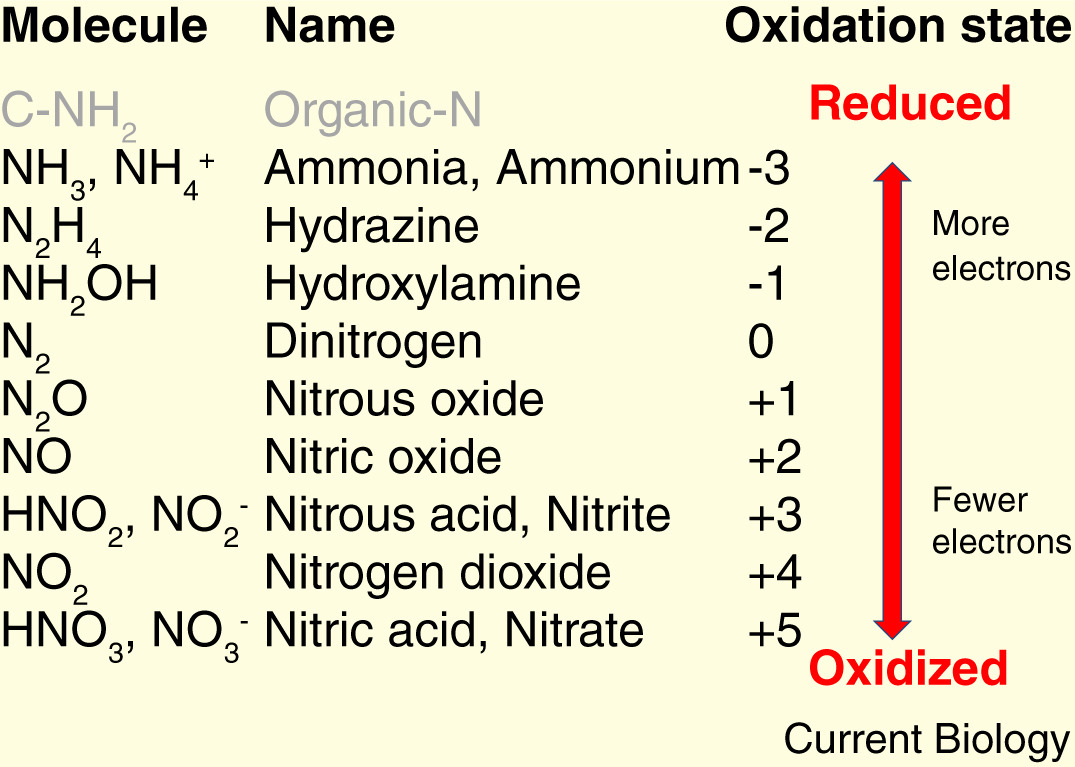
\includegraphics[
        width=0.9\textwidth,
        alt={A diagram showing the nitrogen cycle with different molecules like Ammonia and Nitrite at various oxidation states from -3 to +3.}
        ]
    {images/nitrogen-cycle-intermediates.jpg}
    \caption{Schematic layout of a Waste Stabilization Pond system}
    \label{fig:Nitrogen Cycle}
\end{figure}

\backmatter

\printglossary[type=\acronymtype, title={List of Acronyms}]
\printglossary[title={Glossary}]
\printbibliography[title={References}]


\end{document}